% ═════════════════════════════════════════════════════════════
% L-BFGS Experimental Results
\label{sec:experiments}
% ═════════════════════════════════════════════════════════════

\noindent All experiments use the matrix $X \in \R^{m \times n}$ with $m = 500$ samples and $n = 12$
features after standard preprocessing (zero mean, unit variance per feature).
The response vector $y \in \R^n$ is drawn from a standard normal distribution
with a fixed random seed ($\texttt{seed} = 42$). The reference solution $w^*$
is computed via the normal equations $(XX^T + \lambda^2 I)\,w = Xy$ using
\texttt{numpy.linalg.solve}, with a baseline solve time of approximately
$0.3$\,s.

\noindent Unless stated otherwise, we use the default configuration obtained from a
grid search over the algorithm's hyperparameters (with the initial point
fixed to $w_0 = 0$, the canonical neutral choice): regularization
$\lambda = 0.5$ (yielding $\kappa(\Xhat) = 151.49$), memory size
$\bar{m} = 10$, exact line search, the Barzilai--Borwein $H_0$ scaling
(\texttt{bb1}), and the curvature-based restart enabled. The relative
tolerance is $\varepsilon = 10^{-14}$ unless noted otherwise. Wall-clock
measurements use \texttt{time.perf\_counter()} and report the median over
five repetitions after a discarded warm-up run; reported FLOP counts use the
per-iteration operation model derived in Section~\ref{sec:exp_cost}.

\noindent The experimental discussion is organised in three parts. We first verify the
\emph{theoretical convergence properties} established in
Section~\ref{sec:convergence} (linear and superlinear regimes,
Newton-direction alignment, and a comparison against representative
first-order baselines). We then examine the \emph{algorithmic design choices}
of our L-BFGS variant (line search, memory size, $H_0$ scaling, restart
strategy, Wolfe constants). Finally, we probe the \emph{numerical and
computational behaviour} of the method (sensitivity to initialisation, and
the theoretical FLOP/storage cost together with its scalability in $m$).


% ═════════════════════════════════════════════════════════════
\section{Theoretical Convergence Properties}
\label{sec:exp_theory}
% ═════════════════════════════════════════════════════════════


% ─────────────────────────────────────────────────────────────
\subsection{Empirical Linear and Superlinear Convergence Rates}
\label{sec:exp_rates}
% ─────────────────────────────────────────────────────────────
\noindent We track the convergence behaviour at three memory sizes:
$\bar{m} = 3$ (severely limited), $\bar{m} = 10$ (typical), and
$\bar{m} = m = 500$ (effectively full BFGS, since the algorithm always
converges in fewer than $m$ iterations). We record two per-iteration
quantities: the Q-linear ratio
$r_k^{\mathrm{lin}} = (f_k - f^*)/(f_{k-1} - f^*)$, whose stabilisation at
a constant value below $1$ is the empirical signature of the linear bound
in Eq.~\eqref{eq:linconv}, and the Q-superlinear ratio
$r_k^{\mathrm{sup}} = \norm{w_{k+1} - w^*}/\norm{w_k - w^*}$, whose decay
towards $0$ is the signature of the superlinear regime of
Eq.~\eqref{eq:superlin}.  As in the default
configuration, the curvature-based restart is enabled, and we run at the
tight tolerance $\varepsilon = 10^{-14}$.

\begin{table}[H]
\centering
\caption{L-BFGS at three memory sizes ($\lambda = 0.5$, exact LS,
  restart enabled, $\varepsilon = 10^{-14}$).}
\label{tab:rates}
\small
\setlength{\tabcolsep}{12pt}
\begin{tabular}{cccc}
    \toprule
    $\bar{m}$ & \textbf{Iterations} & $\norm{w - w^*}$ & $f - f^*$ \\
    \midrule
    3   & 287 & $9.43 \times 10^{-11}$ & $2.78 \times 10^{-17}$ \\
    10  & 18  & $5.44 \times 10^{-12}$ & $2.78 \times 10^{-17}$ \\
    500 & 18  & $5.44 \times 10^{-12}$ & $2.78 \times 10^{-17}$ \\
    \bottomrule
\end{tabular}
\end{table}

\begin{figure}[H]
        \centering
        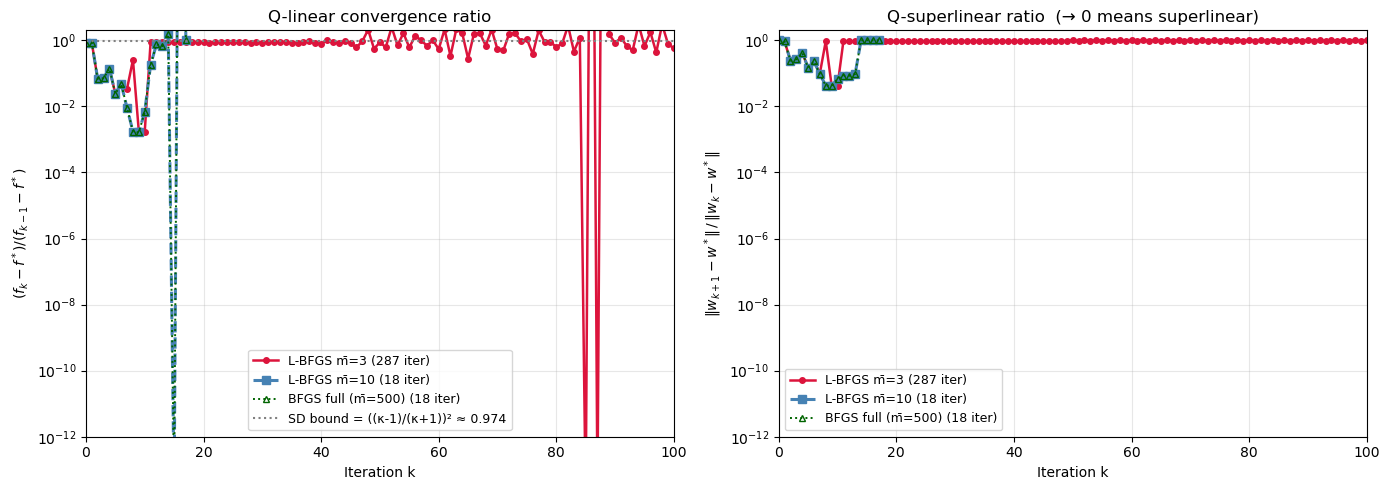
\includegraphics[width=0.80\textwidth]{Chapters/images/convergence_ratios_plot.png}
        \caption{Q-linear (left) and Q-superlinear (right) convergence ratios}
    \end{figure}
    
\noindent The two larger memories, $\bar{m} = 10$ and $\bar{m} = 500$, produce
\emph{identical} trajectories and converge in just $18$ iterations. In the
Q-superlinear panel (right) their ratio descends smoothly to about
$10^{-1}$ before reaching the floor: the stored pairs build a stable,
accurate approximation of the inverse Hessian, so every step is
consistently effective---the behaviour expected of the superlinear regime
of Eq.~\eqref{eq:superlin}. The Q-linear panel (left) shows the
characteristic ``saw-tooth'' of exact line search on a quadratic,
alternating ordinary steps (ratio near $1$) with exceptionally effective
ones (the downward spikes), while always remaining below the
steepest-descent bound $r_{\mathrm{SD}} \approx 0.97$---confirming the
linear bound of Eq.~\eqref{eq:linconv} and that L-BFGS converges far faster
than any first-order method.

\noindent The severely limited memory $\bar{m} = 3$ tells a different story. It
follows the same initial descent but cannot sustain it: with too few
stored pairs, the curvature approximation repeatedly degrades, and the algorithm needs $287$ iterations---over fifteen times more---to reach
the same floor. The restart accelerates this case substantially: without it,
$\bar{m} = 3$ still converges but takes $1{,}147$ iterations, so the restart
yields a roughly fourfold speed-up here (its effect on small memories is
examined in detail in Section~\ref{sec:exp_restart}).

\noindent The contrast between $\bar{m} = 3$ and $\bar{m} \ge 10$ illustrates the
key property of L-BFGS: a small memory matches the full-memory method
\emph{exactly}, provided it exceeds the \emph{effective rank} of the
problem. By Lemma~\ref{lemma:singvals}, $XX^T$ has only $n = 12$ non-zero
eigenvalues, so only $n$ Hessian directions carry non-trivial curvature; a
memory of $\bar{m} \gtrsim n$ captures all of them and any further pairs are
redundant. Storing $10$ vectors is therefore as good as storing all
$500$---and dropping below the effective rank, as with $\bar{m} = 3$,
degrades convergence sharply.


% ─────────────────────────────────────────────────────────────
\subsection{Comparison with Steepest Descent and Conjugate Gradient}
\label{sec:exp_baselines}
% ─────────────────────────────────────────────────────────────

\noindent To assess whether the curvature information used by L-BFGS provides a
practical advantage, we compare it with two natural baselines:
\emph{steepest descent} (SD) with exact line search, and the linear
\emph{conjugate gradient} method (CG) applied to the Symmetric Positive Definite system $Hw = Xy$,
where $H$-vector products are computed implicitly as
$Hv = X(X^Tv) + \lambda^2 v$ at the same $O(mn)$ cost per iteration as L-BFGS.
All methods start from $w_0 = 0$ and use the relative stopping rule
of Eq.~\eqref{eq:stop_rel} with $\varepsilon = 10^{-14}$. Two regimes are
considered: well-conditioned ($\lambda = 1$, $\kappa \approx 76$) and
ill-conditioned ($\lambda = 10^{-4}$, $\kappa \approx 7.6 \times 10^{5}$).

\begin{table}[H]
\centering
\caption{Iteration counts and final gradient norms across four methods
  ($m = 500$, $n = 12$, exact line search, $\varepsilon = 10^{-14}$).}
\label{tab:baselines}
\small
\setlength{\tabcolsep}{12pt}
\begin{tabular}{lcccc}
    \toprule
    & \multicolumn{2}{c}{$\lambda = 1$ ($\kappa \approx 76$)}
    & \multicolumn{2}{c}{$\lambda = 10^{-4}$ ($\kappa \approx 7.6\times10^5$)} \\
    \cmidrule(lr){2-3}\cmidrule(lr){4-5}
    \textbf{Method} & iter & $\norm{\nabla f}$ & iter & $\norm{\nabla f}$ \\
    \midrule
    Steepest Descent           & 1447 & $6.14 \times 10^{-13}$ & 1725 & $6.55 \times 10^{-13}$ \\
    Conjugate Gradient         &   15 & $5.47 \times 10^{-15}$ &   15 & $1.90 \times 10^{-14}$ \\
    L-BFGS ($\bar{m} = 10$)    &   19 & $1.47 \times 10^{-10}$ &   31 & $7.37 \times 10^{-11}$ \\
    Full BFGS ($\bar{m} = 500$)&   19 & $1.47 \times 10^{-10}$ &   31 & $7.37 \times 10^{-11}$ \\
    \bottomrule
\end{tabular}
\end{table}

\begin{figure}[H]
    \centering
    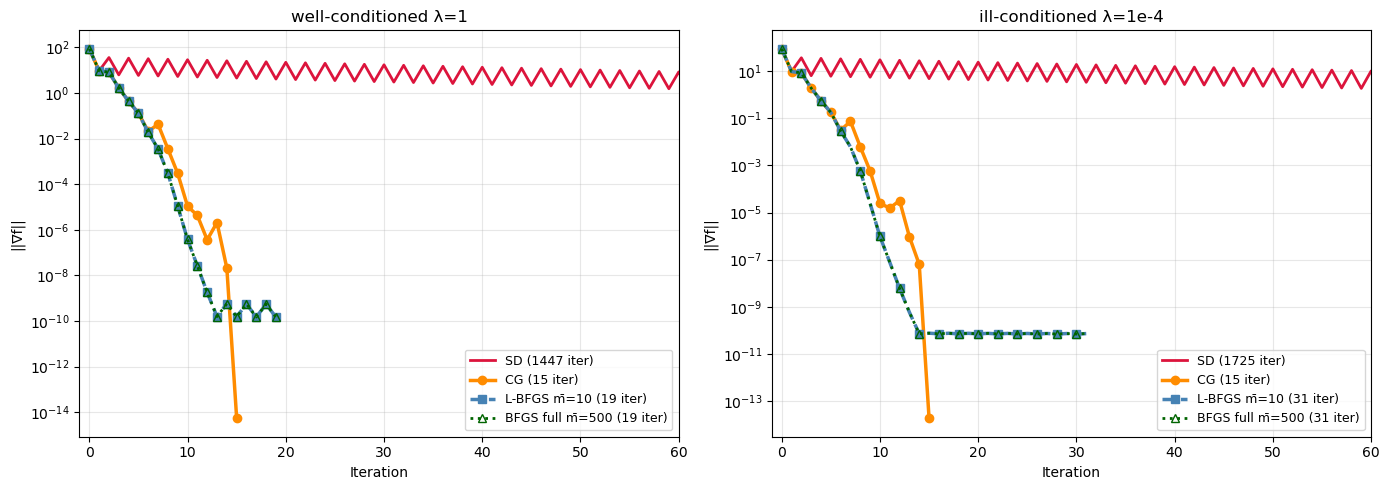
\includegraphics[width=0.80\textwidth]{Chapters/images/comparison_sd_cg.png}
    \caption{Convergence of the four methods ($\norm{\nabla f}$ vs.\
      iteration) in the well-conditioned ($\lambda = 1$, left) and
      ill-conditioned ($\lambda = 10^{-4}$, right) regimes. The $x$-axis is
      truncated at $60$ iterations; SD continues well beyond this range
      (over $1{,}400$ iterations in both cases).}
    \label{fig:baselines}
\end{figure}

\noindent The four methods separate into three performance tiers. Steepest descent
is uncompetitive in both regimes, requiring over $1{,}400$ iterations even
on the well-conditioned problem: using only the gradient, it makes slow
progress along the elongated level sets. L-BFGS with $\bar{m} = 10$ and
full BFGS with $\bar{m} = 500$ produce \emph{identical} trajectories (for
the reason given in Section~\ref{sec:exp_rates}), cutting the iteration
count by nearly two orders of magnitude relative to SD. Conjugate gradient,
however, is faster still, reaching machine precision in just $15$ iterations.

\noindent CG's strong performance is a direct consequence of the problem's algebraic
structure. For SPD systems, CG terminates in a number of iterations equal
to the number of \emph{distinct} eigenvalues of $H$, not its dimension $m$.
As noted in Section~\ref{sec:exp_rates}, $XX^T$ has only $n = 12$ non-zero
eigenvalues (Lemma~\ref{lemma:singvals}); the spectrum of
$H = XX^T + \lambda^2 I$ therefore consists of just $n + 1 = 13$ distinct
values---the $12$ shifted singular values plus $\lambda^2$ with multiplicity
$m - n$. CG resolves this clustered spectrum in roughly $n$ steps regardless
of $\kappa$, which is why it takes $15$ iterations in both regimes.

\noindent Two further effects deserve note. First, conditioning affects L-BFGS but
not CG: raising $\kappa$ from $76$ to $7.6 \times 10^{5}$ increases the
L-BFGS iteration count from $19$ to $31$, while CG stays at $15$. CG's
finite-termination property is immune to $\kappa$, whereas L-BFGS, as a
general quasi-Newton method, is mildly sensitive to it---though far less so
than SD, whose count also grows with $\kappa$ ($1447 \to 1725$). Second, CG
reaches a higher final accuracy ($10^{-14}$--$10^{-15}$ vs.\
$10^{-10}$--$10^{-11}$ for L-BFGS), a consequence of its exact-arithmetic
optimality on quadratics.

\noindent The takeaway is not that L-BFGS is inferior, but that CG wins here precisely
because our problem meets its two ideal assumptions at once: it is
\emph{quadratic} and has a \emph{low-rank, clustered spectrum}. Neither
holds in general---on non-quadratic objectives the conjugacy machinery
breaks down, and on problems with non-clustered spectra CG loses its fast
termination. L-BFGS degrades gracefully in both cases, making it the more
robust choice for the broader class of problems where that structure is
absent.

% ─────────────────────────────────────────────────────────────
\subsection{Alignment with the Newton Direction}
\label{sec:exp_newton}
% ─────────────────────────────────────────────────────────────

\noindent While the previous experiments \emph{observed} superlinear convergence,
this one identifies its \emph{cause}. As anticipated in
Section~\ref{sec:convergence}, Nocedal and
Wright~\cite[Thm.~8.6]{nocedal2006numerical} attribute the superlinear rate
of BFGS to the search direction $p_k = -H_k \nabla f_k$ becoming an
increasingly accurate approximation of the Newton direction
$p_k^{\mathrm{N}} = -H^{-1}\nabla f_k$. We test this directly by measuring
the alignment defect $1 - \cos\theta_k$ between the two directions, using a
cached Cholesky factorisation of $H$ as a measurement oracle. Although this
factorisation costs $O(m^3)$, it is used \emph{only} to compute the
reference Newton direction and is \emph{not} part of the L-BFGS algorithm,
which remains $O(mn + m\bar{m})$ per iteration. To keep the angle
measurement clean, this instrumental variant runs without the
curvature-based restart, so that each trajectory reflects a single,
uninterrupted curvature approximation.

\begin{table}[H]
\centering
\caption{Alignment defect $1 - \cos\theta_k$ at the last \emph{clean}
  iteration (before $\norm{\nabla f}$ reaches the noise floor
  $10^{-9}$).}
\label{tab:newton_angle}
\small
\setlength{\tabcolsep}{12pt}
\begin{tabular}{rcc}
    \toprule
    $\bar{m}$ & \textbf{Clean iterations}
              & \textbf{Final} $1 - \cos\theta_k$ \\
    \midrule
    3        & 40 & $2.83 \times 10^{-1}$ \\
    10, 500  & 13 & $3.53 \times 10^{-3}$ \\
    \bottomrule
\end{tabular}
\end{table}

\noindent The results confirm the mechanism. For $\bar{m} \ge 10$ the defect falls
by two orders of magnitude, reaching $\sim 3.5 \times 10^{-3}$: the L-BFGS
direction becomes nearly indistinguishable from the Newton step, which is
exactly what drives the superlinear regime seen in
Section~\ref{sec:exp_rates}. For $\bar{m} = 3$ the defect stalls at
$\sim 2.8 \times 10^{-1}$ and never improves: with too few stored pairs,
$H_k$ cannot approximate $H^{-1}$ closely enough to recover the Newton
direction. This is the direct cause of its linear-only, much slower
convergence---the $287$ iterations of Section~\ref{sec:exp_rates} are the
price of a search direction that stays misaligned with Newton's. The series
are truncated once $\norm{\nabla f}$ falls below $10^{-9}$, below which both
directions are computed on numerical noise.

\noindent This experiment closes the theoretical loop of
Section~\ref{sec:convergence}: the superlinear convergence of large-memory
BFGS, the linear-only convergence of severely limited L-BFGS, and the
iteration counts of Sections~\ref{sec:exp_rates}
and~\ref{sec:exp_baselines} are all manifestations of the same underlying
mechanism---the quality of the curvature approximation built by the
two-loop recursion.

%% TODO: insert (1 - cos theta_k) vs iter plot, with floor masked

% ═════════════════════════════════════════════════════════════
\section{Algorithmic Design Choices}
\label{sec:exp_design}
% ═════════════════════════════════════════════════════════════

\noindent Each experiment in this section isolates a single design decision in our
L-BFGS implementation and quantifies its impact on convergence. Together,
these experiments justify the default configuration used in the remainder
of the chapter (\texttt{line\_search='exact'}, $\bar{m} = 10$,
\texttt{h0\_scaling='bb1'}, \texttt{use\_restart=True}, $\xi = 0.2$).


% ─────────────────────────────────────────────────────────────
\subsection{Exact Line Search vs.\ Strong Wolfe Line Search}
\label{sec:exp_exact_vs_wolfe}
% ─────────────────────────────────────────────────────────────

\noindent We compare the two line-search strategies at a tight relative tolerance
$\varepsilon = 10^{-14}$, using the standard Wolfe constants
$(c_1, c_2) = (10^{-4}, 0.9)$ recommended by Nocedal and
Wright~\cite[Sec.~3.1]{nocedal2006numerical} for quasi-Newton methods.

\begin{table}[H]
\centering
\caption{Comparison of line-search strategies
  ($m = 500$, $n = 12$, $\lambda = 0.5$, $\bar{m} = 10$,
  $\varepsilon = 10^{-14}$).}
\label{tab:ls_comparison}
\small
\setlength{\tabcolsep}{10pt}
\begin{tabular}{lcccc}
    \toprule
    \textbf{Line Search} & \textbf{Iterations} & $\norm{w - w^*}$
      & \textbf{Time (s)} & \textbf{Stop reason} \\
    \midrule
    Exact   & 18  & $5.44 \times 10^{-12}$ & 0.001 & stagnation \\
    Wolfe ($c_1=10^{-4}, c_2=0.9$) & 599 & $5.21 \times 10^{-8}$ & 0.023 & stagnation \\
    \bottomrule
\end{tabular}
\end{table}

\noindent Exact LS achieves nearly four orders of magnitude higher accuracy
($5.4 \times 10^{-12}$ vs.\ $5.2 \times 10^{-8}$) in only $18$ iterations,
against the $599$ that Wolfe needs before stalling. Its closed-form
minimiser, Eq.~\eqref{eq:exact_alpha_expanded}, exploits the quadratic
structure perfectly at the cost of a single matrix-vector product
$X^T p_k \in O(mn)$.

\noindent The Wolfe variant does not diverge but \emph{stalls}: after roughly the
first $100$ iterations the step length stabilises around
$\alpha \approx 0.07$, too large to trigger the stagnation safeguard but too
small for the curvature condition to extract further progress. The cubic
interpolation inside the bracketing-and-zoom loop loses accuracy once
$\norm{\nabla f} \lesssim 10^{-5}$, the working precision of the line search
itself, and the run eventually stops on stagnation at $599$ iterations.

\noindent An important caveat is that the Wolfe defaults
$(c_1, c_2) = (10^{-4}, 0.9)$ are the standard recommendation for
\emph{non-quadratic} quasi-Newton problems. The next experiment shows that
this default is inappropriate for our quadratic structure: with a stricter
$c_2$, Wolfe LS becomes competitive again.

%% TODO: insert convergence plot (Figure: Exact vs Wolfe, ||grad|| and f vs iter)


% ─────────────────────────────────────────────────────────────
\subsection{Sensitivity to the Wolfe Constants $c_1, c_2$}
\label{sec:exp_wolfe_constants}
% ─────────────────────────────────────────────────────────────

\noindent Building on the previous experiment, we test whether the poor performance of
Wolfe LS is intrinsic or a side effect of the standard $c_2 = 0.9$. We
sweep $c_1 \in \{10^{-4}, 10^{-3}, 10^{-2}\}$ and $c_2 \in \{0.1, \dots, 0.9\}$, recording iterations and final accuracy.

\begin{table}[H]
\centering
\caption{Effect of the Wolfe constants on convergence
  ($m = 500$, $n = 12$, $\lambda = 0.5$, $\bar{m} = 10$,
  $\varepsilon = 10^{-14}$). The three $c_1$ columns are identical,
  confirming that $c_1$ has no effect.}
\label{tab:wolfe_sweep}
\small
\setlength{\tabcolsep}{12pt}
\begin{tabular}{ccccc}
    \toprule
    & \multicolumn{3}{c}{\textbf{Iterations} (by $c_1$)} & \\
    \cmidrule(lr){2-4}
    $c_2$ & $10^{-4}$ & $10^{-3}$ & $10^{-2}$ & $\norm{w - w^*}$ \\
    \midrule
    0.1 & 613 & 613 & 613 & $6.54 \times 10^{-8}$ \\
    0.3 & 26  & 26  & 26  & $1.27 \times 10^{-9}$ \\
    0.5 & 25  & 25  & 25  & $1.88 \times 10^{-9}$ \\
    0.7 & 31  & 31  & 31  & $2.11 \times 10^{-9}$ \\
    0.9 & 599 & 599 & 599 & $5.21 \times 10^{-8}$ \\
    \bottomrule
\end{tabular}
\end{table}

\noindent Two observations stand out. First, $c_1$ has \emph{no} effect: all three
values produce identical iteration counts and accuracies. The Armijo
condition is loose enough to be automatically satisfied at the
curvature-determined trial step, so $c_1$ is structurally inactive here.

\noindent Second, and more interestingly, the dependence on $c_2$ is
\emph{non-monotone}: Wolfe LS performs well across a \emph{broad} interior
range and fails only at the two extremes. For $c_2 \in [0.2, 0.8]$ it
converges in roughly $22$--$34$ iterations---competitive with exact LS
($18$)---whereas both $c_2 = 0.1$ and $c_2 = 0.9$ collapse to $\sim 600$
iterations. The two failures have opposite causes. A large $c_2 = 0.9$ makes
the curvature condition too permissive: it accepts steps that barely reduce
the directional derivative, yielding poor curvature pairs and slow progress.
A small $c_2 = 0.1$ makes it too restrictive: the line search struggles to
locate a step tight enough to satisfy it, and the cubic interpolation
stalls before doing so. Only an intermediate $c_2$ balances the two.

\noindent This experiment reframes the conclusion of
Section~\ref{sec:exp_exact_vs_wolfe}: the apparent ``Wolfe failure'' was
caused entirely by the default $c_2 = 0.9$ landing on a bad extreme. With an
intermediate value such as $c_2 = 0.5$, Wolfe LS converges in $25$
iterations---competitive with, though still slightly slower than, exact LS
at $18$ iterations.

%% TODO: insert convergence plot (||grad|| vs iter, colour = c2, linestyle = c1)


% ─────────────────────────────────────────────────────────────
\subsection{Effect of the Memory Parameter $\bar{m}$}
\label{sec:exp_memory}
% ─────────────────────────────────────────────────────────────

\noindent We vary $\bar{m} \in \{3, 5, 10, 20, 40\}$ using exact line search at the
tight tolerance $\varepsilon = 10^{-14}$, with the curvature-based restart
enabled (as in the default configuration).

\begin{table}[H]
\centering
\caption{Effect of memory size $\bar{m}$ on L-BFGS convergence
  ($m = 500$, $n = 12$, $\lambda = 0.5$, exact LS, restart enabled,
  $\varepsilon = 10^{-14}$).}
\label{tab:memory_effect}
\small
\setlength{\tabcolsep}{12pt}
\begin{tabular}{rcc}
    \toprule
    $\bar{m}$ & \textbf{Iterations} & $\norm{w - w^*}$ \\
    \midrule
    3   & 287 & $9.43 \times 10^{-11}$ \\
    5   & 605 & $2.76 \times 10^{-10}$ \\
    10  & 18  & $5.44 \times 10^{-12}$ \\
    20  & 18  & $5.44 \times 10^{-12}$ \\
    40  & 18  & $5.44 \times 10^{-12}$ \\
    \bottomrule
\end{tabular}
\end{table}

\begin{figure}[H]
    \centering
    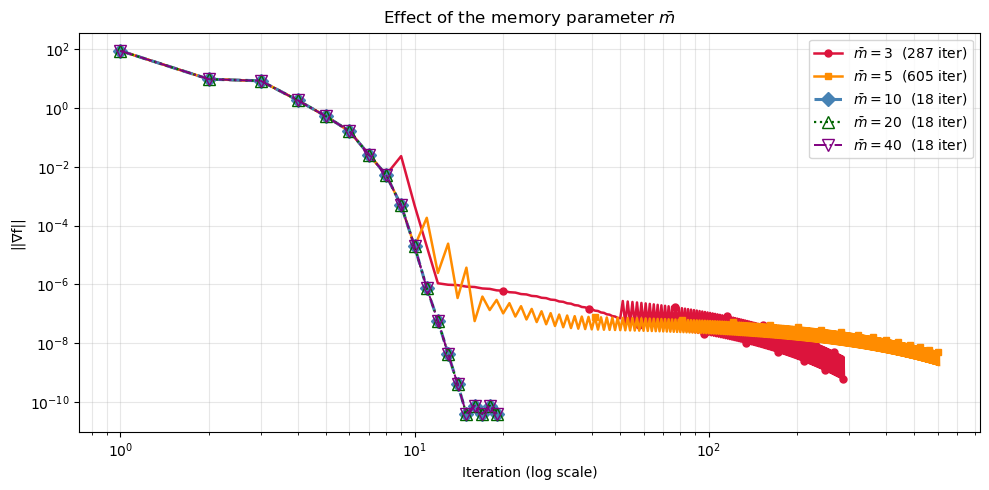
\includegraphics[width=0.70\textwidth]{Chapters/images/memory_effect.png}
    \caption{Gradient-norm convergence for $\bar{m} \in \{3, 5, 10, 20, 40\}$
  (log--log scale, iteration counts in the legend). The curves for
  $\bar{m} \ge 10$ overlap and reach the floor in $18$ iterations. Note the
  non-monotonicity: $\bar{m} = 5$ (orange) lies \emph{above} $\bar{m} = 3$
  (red), taking more than twice as many iterations despite using more
  memory.}
    \label{fig:memory_effect}
\end{figure}

\noindent From $\bar{m} = 10$ onwards the iteration count saturates at $18$ and the
accuracy plateaus at $\norm{w - w^*} \approx 5.4 \times 10^{-12}$. This is the same rank-saturation effect established in
Section~\ref{sec:exp_rates}: a memory of $\bar{m} \gtrsim n = 12$ captures
all the non-trivial curvature directions, so $\bar{m} = 10$, $20$, and $40$
are indistinguishable.

\noindent More striking is the \emph{non-monotone} behaviour at small $\bar{m}$:
$\bar{m} = 3$ takes $287$ iterations, yet $\bar{m} = 5$---with \emph{more}
memory---takes $605$, more than twice as many. This is the documented
non-monotone dependence of L-BFGS on memory
size~\cite[Sec.~9.1]{nocedal2006numerical}: for certain $\bar{m}$ below the
effective rank $n = 12$, the stored curvature pairs interact unfavourably
with the true Hessian spectrum, slowing convergence without affecting the
final accuracy. Adding memory in this regime is no guarantee of faster
convergence, since a larger but still-deficient set of pairs can distort the
search direction more than a smaller one. The practical recommendation is
therefore to set $\bar{m} \gtrsim n$, comfortably above this irregular
regime.

\noindent The small-memory configurations are also where the curvature-based
restart has its strongest effect. At the default $\bar{m} = 10$ the restart
is dormant (it changes nothing), but at $\bar{m} = 3$ it speeds up
convergence appreciably---from $1{,}147$ to $287$ iterations at
$\lambda = 0.5$. Its effect in this regime is, however, not uniformly
beneficial across conditioning; we return to this in
Section~\ref{sec:exp_restart}.

%% TODO: insert plot (||grad|| vs iter on log-x scale, with iter counts in legend)


% ─────────────────────────────────────────────────────────────
\subsection{Effect of the Regularization Parameter $\lambda$}
\label{sec:exp_lambda}
% ─────────────────────────────────────────────────────────────

\noindent We study convergence across five regularization regimes. Recall from
Eq.~\eqref{eq:condition} that $\kappa(\Xhat)$ scales as $O(1/\lambda)$ for
small $\lambda$: weak regularization produces an ill-conditioned, elongated
landscape, while large $\lambda$ drives $\kappa(\Xhat) \to 1$, making the
problem nearly spherical.

\begin{table}[H]
\centering
\caption{Effect of $\lambda$ on condition number and convergence
  ($m = 500$, $n = 12$, exact LS, $\bar{m} = 10$, $\varepsilon = 10^{-14}$).}
\label{tab:lambda_effect}
\small
\setlength{\tabcolsep}{12pt}
\begin{tabular}{lcccc}
    \toprule
    $\lambda$ & $\kappa(\Xhat)$ & \textbf{Iter}
      & $\norm{w - w^*}$ & $t_{\mathrm{LBFGS}}$ (ms) \\
    \midrule
    $10^{-4}$ & $7.6 \times 10^{5}$ & 31 & $1.11 \times 10^{-5}$  & 1.23 \\
    $10^{-2}$ & $7.6 \times 10^{3}$ & 15 & $1.11 \times 10^{-9}$  & 0.69 \\
    $1$       & $75.8$              & 19 & $1.81 \times 10^{-11}$ & 1.01 \\
    $10^{2}$  & $1.3$               &  6 & $3.26 \times 10^{-18}$ & 0.59 \\
    $10^{4}$  & $1.0$               &  3 & $3.99 \times 10^{-22}$ & 0.09 \\
    \bottomrule
\end{tabular}
\end{table}

% \begin{figure}[H]
%     \centering
%     \includegraphics[width=0.75\textwidth]{Chapters/images/lambda_effect_plot.png}
%     \caption{Gradient-norm convergence for five values of $\lambda$.
%       Smaller $\lambda$ (higher $\kappa$) yields a shallower slope; the
%       near-spherical cases $\lambda \ge 10^2$ converge in $3$--$6$ steps.}
%     \label{fig:lambda_effect}
% \end{figure}


\noindent Three observations emerge. First, the iteration count stays small and only
weakly dependent on conditioning: it ranges from $15$ to $31$ across the
three ill- to moderately-conditioned regimes ($\kappa$ from $76$ to
$7.6 \times 10^{5}$), without growing monotonically with $\kappa$. This
confirms that L-BFGS with exact LS converges in $O(n)$ iterations largely
independent of $\kappa$, consistent with the conjugate-direction
interpretation of memoryless BFGS \cite[Sec.~9.1]{nocedal2006numerical} and
with the rank-$12$ structure of $XX^T$ (Lemma~\ref{lemma:singvals}).

\noindent Second, although the iteration count stays low, \emph{final accuracy
degrades sharply with $\kappa$}: from $4 \times 10^{-22}$ at
$\lambda = 10^{4}$ to $1.1 \times 10^{-5}$ at $\lambda = 10^{-4}$. This is
not a failure of the algorithm but the intrinsic floating-point floor of the
normal-equations formulation: forming $XX^T$ squares the condition number
(Eq.~\eqref{eq:Xhat_gram}), so the attainable error is bounded below by
roughly $\kappa^2 \cdot \varepsilon_{\mathrm{mach}}$. At $\lambda = 10^{-4}$
this gives ${\sim}10^{-4}$, consistent with the observed
$1.1 \times 10^{-5}$.

\noindent Third, in the regime $\lambda \gg \sigma_{\max}(X)$ the regularisation term
dominates, $H \approx \lambda^2 I$, and L-BFGS reduces to scaled gradient
descent on a near-spherical problem, converging in $3$--$6$ iterations.
Across all regimes L-BFGS solves the problem in about $1$\,ms.
Section~\ref{sec:exp_cost} examines how this cost scales with $m$.

\noindent Finally, this experiment clarifies why we adopt $\lambda = 0.5$ as the
default for the rest of the chapter. The parameter $\lambda$ is not an
algorithmic knob but part of the problem definition: it sets the
regularisation strength, and hence the trade-off between fitting the data
and controlling $\norm{w}$. Although large $\lambda$ makes the problem
numerically trivial (the case $\lambda = 10^4$ converges in $3$ iterations
to machine precision), the resulting solution is dominated by the penalty
term $\lambda^2\norm{w}^2$ and is essentially $w \approx 0$, ignoring the
data entirely. The value $\lambda = 0.5$ instead yields a moderately
ill-conditioned instance ($\kappa \approx 151$) that is representative of
realistic regularisation and exercises the algorithm in its non-trivial
regime---neither so well-conditioned that convergence is immediate, nor so
ill-conditioned that the problem becomes numerically unsolvable.

%% TODO: insert plot (||grad|| vs iter for the 5 lambda values)


% ─────────────────────────────────────────────────────────────
\subsection{$H_0$ Scaling Strategies}
\label{sec:exp_h0}
% ─────────────────────────────────────────────────────────────

\noindent We compare the three strategies introduced in
Section~\ref{sec:h0_scaling} for the initial Hessian approximation
$H_k^0 = \gamma_k I$ used in the two-loop recursion: the Nocedal default
(BB2, Eq.~\eqref{eq:gamma_nocedal}), the Barzilai--Borwein companion
(BB1, Eq.~\eqref{eq:gamma_bb1}), and the safeguarded variant. To show that the comparison does not depend on
the restart, we run each strategy both with and without it, in both
conditioning regimes.

\begin{table}[H]
\centering
\caption{Effect of $H_0$ scaling on L-BFGS convergence, with and without the
  curvature-based restart ($m = 500$, $n = 12$, exact LS, $\bar{m} = 10$,
  $\varepsilon = 10^{-14}$).}
\label{tab:h0_scaling}
\small
\setlength{\tabcolsep}{9pt}
\begin{tabular}{llcccc}
    \toprule
    & & \multicolumn{2}{c}{\emph{Well-cond.} ($\lambda = 1$, $\kappa \approx 76$)}
      & \multicolumn{2}{c}{\emph{Ill-cond.} ($\lambda = 10^{-2}$, $\kappa \approx 7.6\times10^3$)} \\
    \cmidrule(lr){3-4}\cmidrule(lr){5-6}
    \textbf{Strategy} & \textbf{Restart} & iter & $\norm{w - w^*}$
                                         & iter & $\norm{w - w^*}$ \\
    \midrule
    \texttt{nocedal}     & off & 38 & $3.82\times10^{-12}$ & 29 & $1.11\times10^{-9}$ \\
    \texttt{nocedal}     & on  & 38 & $3.82\times10^{-12}$ & 29 & $1.11\times10^{-9}$ \\
    \texttt{bb1}         & off & 19 & $1.81\times10^{-11}$ & 15 & $1.11\times10^{-9}$ \\
    \texttt{bb1}         & on  & 19 & $1.81\times10^{-11}$ & 15 & $1.11\times10^{-9}$ \\
    \texttt{safeguarded} & off & 38 & $3.82\times10^{-12}$ & 29 & $1.11\times10^{-9}$ \\
    \texttt{safeguarded} & on  & 38 & $3.82\times10^{-12}$ & 29 & $1.11\times10^{-9}$ \\
    \bottomrule
\end{tabular}
\end{table}

\noindent Two clear results emerge. First, \texttt{bb1} converges in roughly
\emph{half} the iterations of the other two strategies---$19$ vs.\ $38$ in
the well-conditioned regime, $15$ vs.\ $29$ in the ill-conditioned one---and
this gap is \emph{identical with and without the restart}, confirming that
it is a genuine property of the scaling rule rather than an interaction with
the restart. The two BB formulas are related by the Cauchy--Schwarz
inequality, which gives $\gamma^{\mathrm{BB1}} \ge \gamma^{\mathrm{N}}$: the
larger initial scale of \texttt{bb1} produces more effective early steps on
this problem, at the cost of a marginally higher final residual
($1.8 \times 10^{-11}$ vs.\ $3.8 \times 10^{-12}$, both at the floor). This
advantage is exactly what led the grid search to select \texttt{bb1} as the
default.

\noindent Second, \texttt{nocedal} and \texttt{safeguarded} produce
\emph{identical} results to the last digit. The safeguard clips $\gamma$
into a safe interval to prevent it from exploding near the solution (where
$y^Ty \to 0$), but on this well-behaved quadratic $\gamma$ never approaches
the clipping bounds, so the safeguard never activates. It is thus free
insurance---inert here, but a cheap guarantee of robustness on problems
where $\gamma$ might otherwise degenerate.

%% TODO: insert convergence plot (3 strategies, two regimes, distinguishable styles)


% ─────────────────────────────────────────────────────────────
\subsection{Curvature-Based Restart}
\label{sec:exp_restart}
% ─────────────────────────────────────────────────────────────

\noindent The curvature-based restart of Liu and
Nocedal~\cite[Sec.~4]{liu1989limited} clears the L-BFGS memory whenever the
curvature ratio $\gamma_k = (s^Ty)/(y^Ty)$ drops by more than a factor
$\xi$ relative to the previous iteration (Eq.~\eqref{eq:restart_cond}),
signalling entry into a region of qualitatively different curvature. We test
it against a no-restart control at two memory sizes: the default
$\bar{m} = 10$ and the severely limited $\bar{m} = 3$, in both conditioning
regimes.

\begin{table}[H]
\centering
\caption{Effect of the curvature-based restart ($\xi = 0.20$) at two memory
  sizes ($m = 500$, $n = 12$, exact LS, \texttt{bb1},
  $\varepsilon = 10^{-14}$).}
\label{tab:restart_effect}
\small
\setlength{\tabcolsep}{9pt}
\begin{tabular}{llcccc}
    \toprule
    & & \multicolumn{2}{c}{\emph{Well-cond.} ($\lambda = 1$)}
      & \multicolumn{2}{c}{\emph{Ill-cond.} ($\lambda = 10^{-2}$)} \\
    \cmidrule(lr){3-4}\cmidrule(lr){5-6}
    $\bar{m}$ & \textbf{Restart} & iter & n\_memory\_clears & iter & n\_memory\_clears \\
    \midrule
    10 & off          & 19  & 1 & 15  & 1 \\
    10 & $\xi = 0.20$  & 19  & 1 & 15  & 1 \\
    \midrule
    3  & off          & 897 & 1 & 332 & 1 \\
    3  & $\xi = 0.20$  & 399 & 3 & 848 & 3 \\
    \bottomrule
\end{tabular}
\end{table}

\noindent The two memory sizes tell opposite stories. With the default
$\bar{m} = 10$ the restart is \emph{dormant}: enabling it leaves the
iteration count unchanged in both regimes ($19$ and $15$). The single
memory clear counted in these runs is not the $\xi$-test at all, but the
negative-curvature reset triggered when $y^Ts$ becomes negligibly small near
the floor (cf.\ Section~\ref{sec:restart}). A sweep over
$\xi \in \{0.05, 0.10, 0.20, 0.40, 0.70\}$ confirms this: all five
thresholds give identical results ($15$ iterations), so the $\xi$-test never
fires when the memory is adequate.
% [DATA] sweep xi conferma dormant a m=10

\noindent The reason is structural. The objective is quadratic, so $H$ is constant
and $\gamma_k$ (Eq.~\eqref{eq:gamma_restart}) stays bounded between
$1/\lambda_{\max}(H)$ and $1/\lambda_{\min}(H)$. With $\bar{m} \ge n$ the
curvature approximation is stable throughout, so $\gamma_k$ never drops by
the factor required to trigger a reset. The mechanism is therefore inert at
the default memory size, adding only negligible overhead.

\noindent With the starved $\bar{m} = 3$, by contrast, the $\xi$-test \emph{does}
fire (three resets in each run), and its effect is substantial but
\emph{not uniformly beneficial}. In the well-conditioned regime it more than
halves the iteration count ($897 \to 399$), as clearing the stale,
rank-deficient memory lets the method rebuild a fresher curvature estimate.
In the ill-conditioned regime, however, it makes matters \emph{worse}
($332 \to 848$): here the discarded pairs, though imperfect, still carried
useful low-curvature information, and rebuilding from scratch repeatedly
costs more than it saves. The restart thus trades stale information for
freshness---a trade that pays off only when the stale information is
genuinely harmful.
% [DATA/STORY] m=3: aiuta well (897->399), peggiora ill (332->848); onesto

\noindent For our purposes the conclusion is clear. At the default $\bar{m} = 10$ the
restart is inactive and costless, so we leave it enabled as a no-risk
safeguard: it never interferes when the memory is adequate, and remains
available should a smaller memory be used. Its variable behaviour at
$\bar{m} = 3$ is a further argument for choosing $\bar{m} \gtrsim n$, where the question does not arise.

% ═════════════════════════════════════════════════════════════
\section{Numerical and Computational Scalability}
\label{sec:exp_scalability}
% ═════════════════════════════════════════════════════════════

\noindent The previous sections established the theoretical and algorithmic behaviour
of L-BFGS on the default ML-CUP instance. We now probe two remaining
practical aspects: how robust the method is to the choice of starting
point, what its theoretical computational cost is, and how it scales empirically
with the problem dimensions $n$ and $m$.

% ─────────────────────────────────────────────────────────────
\subsection{Sensitivity to the Initial Iterate $w_0$}
\label{sec:exp_init}
% ─────────────────────────────────────────────────────────────

\noindent As established in Section~\ref{sec:convergence}, L-BFGS converges from any
starting point on a strongly convex quadratic, with a rate depending only
on $\kappa$. We test four starting points spanning four orders of magnitude
in $\norm{w_0 - w^*}$, from $w_0 = 0$ to a point at distance ${\sim}2{,}000$,
plus one deliberately placed very close to the optimum.

\begin{table}[H]
\centering
\caption{Sensitivity to the initial iterate
  ($m = 500$, $n = 12$, $\lambda = 0.5$, $\bar{m} = 10$, exact LS,
  $\varepsilon = 10^{-14}$).}
\label{tab:init_sensitivity}
\small
\setlength{\tabcolsep}{12pt}
\begin{tabular}{lrcc}
    \toprule
    \textbf{Initialization} & $\norm{w_0 - w^*}$
      & \textbf{Iter} & $\norm{w - w^*}$ \\
    \midrule
    \texttt{zeros}                & $0.85$               & 18 & $5.44 \times 10^{-12}$ \\
    \texttt{random N(0, 1)}       & $22.0$               & 18 & $1.91 \times 10^{-12}$ \\
    \texttt{random N(0, $100^2$)} & $2.19 \times 10^{3}$ & 15 & $1.13 \times 10^{-12}$ \\
    \texttt{near optimum} ($w^* + 0.01 \cdot \mathcal{N}(0,1)$)
                                  & $0.23$               & 41 & $2.83 \times 10^{-12}$ \\
    \bottomrule
\end{tabular}
\end{table}

\noindent The main result is that the \emph{distance} to the optimum does not
determine the iteration count. The three generic starts converge in
$15$--$18$ iterations even though $\norm{w_0 - w^*}$ ranges over four orders
of magnitude; remarkably, the \emph{farthest} start (\texttt{N(0, $100^2$)},
at distance ${\sim}2{,}200$) converges in the \emph{fewest} iterations
($15$). This is the global linear convergence guarantee of
Eq.~\eqref{eq:linconv} in action: on a strongly convex quadratic the rate
depends only on $\kappa$, not on $w_0$. The slight edge of the far start is
a minor geometric effect---a generic point off the origin produces richer
initial curvature pairs than the structured choice $w_0 = 0$---and it is
precisely this artefact that led the grid search to rank random
initialisations marginally above \texttt{zeros}; we nonetheless fix
$w_0 = 0$ as the canonical neutral default.

\noindent The \texttt{near optimum} start is the apparent exception: despite being
the \emph{closest} ($\norm{w_0 - w^*} = 0.23$), it takes the \emph{most}
iterations ($41$). This does not contradict the global convergence result;
it is an artefact of the \emph{relative} stopping criterion
(Eq.~\eqref{eq:stop_rel}). Starting near $w^*$ gives a small initial
gradient $\norm{\nabla f_0}$, so the absolute threshold
$\varepsilon \cdot \norm{\nabla f_0}$ becomes proportionally tighter, and
more iterations are needed to squeeze out the extra orders of magnitude. The
difficulty lies in the convergence \emph{measure}, not in the problem
itself: the final accuracy ($2.8 \times 10^{-12}$) is the same as the other
starts.


% ─────────────────────────────────────────────────────────────
\subsection{Theoretical Cost, Storage, and Scalability}
\label{sec:exp_cost}
% ─────────────────────────────────────────────────────────────

\noindent The main practical motivation for L-BFGS is its favourable cost compared
with a direct solver. Forming and factorising the normal equations
$(XX^T + \lambda^2 I)\,w = Xy$ with \texttt{numpy.linalg.solve} costs
$O(m^3)$, whereas L-BFGS costs $O\big((mn + m\bar{m})\, n_{\mathrm{iter}}\big)$,
with $n_{\mathrm{iter}}$ governed by the conditioning and effective rank
rather than by $m$. We make this concrete with a FLOP count derived from the
structure of the two-loop recursion (Algorithm~\ref{alg:twoloop}). Per
iteration,
\[
  \text{FLOPs/iter} = \underbrace{(4\bar{m} + 1)\,m}_{\text{two-loop}}
                    + \underbrace{2mn}_{\text{gradient}}
                    + \underbrace{mn + 2m}_{\text{exact LS}}
                    + \underbrace{2m}_{\text{update}},
\]
which is linear in both $m$ and $\bar{m}$, while storage is
$2\bar{m}$ vectors of length $m$ plus $O(m)$ working space. Crucially, the
\emph{total} cost to convergence depends on both this per-iteration work
\emph{and} the iteration count, which combine non-trivially.

\begin{table}[H]
\centering
\caption{Total FLOPs to convergence vs.\ $\bar{m}$
  ($m = 500$, $n = 12$, $\lambda = 0.5$, exact LS, $\varepsilon = 10^{-14}$).
  Iteration counts are those of Table~\ref{tab:memory_effect}.}
\label{tab:total_flops}
\small
\setlength{\tabcolsep}{12pt}
\begin{tabular}{rrrrr}
    \toprule
    $\bar{m}$ & \textbf{Iter} & \textbf{FLOPs/iter}
      & \textbf{Total FLOPs} & \textbf{Storage (MB)} \\
    \midrule
    3   & 287 & $26{,}500$  & $7{,}605{,}500$  & 0.040 \\
    5   & 605 & $30{,}500$  & $18{,}452{,}500$ & 0.056 \\
    10  & 18  & $40{,}500$  & $729{,}000$      & 0.096 \\
    20  & 18  & $60{,}500$  & $1{,}089{,}000$  & 0.176 \\
    40  & 18  & $100{,}500$ & $1{,}809{,}000$  & 0.336 \\
    \bottomrule
\end{tabular}
\end{table}

\noindent The total cost is strongly \emph{non-monotone} in $\bar{m}$, driven entirely
by the iteration count of Section~\ref{sec:exp_memory}. The configuration
$\bar{m} = 5$ requires $18.5$M FLOPs---over $25\times$ more than the optimal
$\bar{m} = 10$ at $0.73$M---and even $\bar{m} = 3$ ($7.6$M) outperforms it,
a direct FLOP-level manifestation of the rank-deficient Hessian structure.
The sweet spot is $\bar{m} = 10$: just above the effective rank, it captures
the relevant curvature with minimal redundancy. Increasing $\bar{m}$ further
only inflates the per-iteration cost without reducing the iteration count,
so the total grows linearly beyond this point. Storage is never a
constraint: even $\bar{m} = 40$ uses only $0.34$\,MB, so $\bar{m}$ should be
chosen for convergence speed alone.

\noindent Returning to the comparison with the direct solver, the FLOP model makes
the asymptotic advantage explicit. At the optimal $\bar{m} = 10$, L-BFGS
needs about $0.73$M FLOPs on the present ML-CUP instance ($m=500$). More
generally, if the iteration count remains roughly constant, the total cost
scales approximately linearly in $m$, since each iteration costs
$O(mn + m\bar{m})$. The direct solver, by contrast, scales as $O(m^3)$. For
the ML-CUP dimensions this gap is already substantial, and it widens by a
further factor of about $m^2$ as the problem size grows, which is precisely
the regime where the limited-memory approach becomes indispensable. We verify this scaling empirically---and confirm the
governing role of the effective rank $n$---in Section~\ref{sec:exp_scaling_nm}.


% ─────────────────────────────────────────────────────────────
\subsection{Empirical Scaling with the Dimensions $n$ and $m$}
\label{sec:exp_scaling_nm}
% ─────────────────────────────────────────────────────────────

\noindent The cost analysis above, like all preceding experiments, is based on the
fixed ML-CUP matrix ($m = 500$, $n = 12$). To verify directly how the method
scales with the problem dimensions---and, in particular, to confirm that the
iteration count is governed by the effective rank $n$ rather than by the
sample size $m$---we run two sweeps on synthetic Gaussian data with
standardised columns. We report only iteration counts (which are
deterministic and noise-free) together with $\kappa(\Xhat)$, computed exactly
from the singular values of $X$; this separates the effect of \emph{dimension}
from that of \emph{conditioning}.

\begin{table}[H]
\centering
\caption{Scaling with the number of features $n$ (fixed $m = 500$, exact LS,
  \texttt{bb1}, $\varepsilon = 10^{-14}$). The saturation memory
  $\bar{m}^*$ is the smallest $\bar{m}$ reaching the iteration plateau.}
\label{tab:scaling_n}
\small
\setlength{\tabcolsep}{12pt}
\begin{tabular}{rrrrr}
    \toprule
    $n$ & $\kappa(\Xhat)$ & \textbf{iter L-BFGS}
        & \textbf{iter CG} & $\bar{m}^*$ \\
    \midrule
    5   & 1.17 & 5  & 5  & 3  \\
    12  & 1.28 & 18 & 12 & 10 \\
    25  & 1.50 & 19 & 18 & 23 \\
    50  & 1.84 & 33 & 25 & 48 \\
    100 & 2.46 & 48 & 36 & 98 \\
    \bottomrule
\end{tabular}
\end{table}

% \begin{figure}[H]
%     \centering
%     \includegraphics[width=0.70\textwidth]{Chapters/images/scaling_n.png}
%     \caption{Scaling with the number of features $n$ at fixed $m = 500$ and
%       nearly constant conditioning ($\kappa$ between $1.2$ and $2.5$). The
%       saturation memory $\bar{m}^*$ (red) tracks the reference line $y = n$
%       almost exactly, confirming that the memory required to reach the
%       iteration plateau is the effective rank; CG terminates in at most $n$
%       steps (orange), and the L-BFGS count (blue) grows in step. All three
%       indicators scale with $n$, not with $m$.}
%     \label{fig:scaling_n}
% \end{figure}

\begin{table}[H]
\centering
\caption{Scaling with the sample size $m$ (fixed $n = 12$, exact LS,
  \texttt{bb1}, $\varepsilon = 10^{-14}$).}
\label{tab:scaling_m}
\small
\setlength{\tabcolsep}{12pt}
\begin{tabular}{rrrr}
    \toprule
    $m$ & $\kappa(\Xhat)$ & \textbf{iter L-BFGS} & \textbf{iter CG} \\
    \midrule
    200  & 1.45 & 21 & 12 \\
    500  & 1.28 & 18 & 12 \\
    2000 & 1.15 & 14 & 11 \\
    8000 & 1.06 & 10 &  9 \\
    \bottomrule
\end{tabular}
\end{table}

\noindent The two sweeps confirm the central structural claim of this chapter: the
convergence of both methods is governed by the effective rank $n$, not by the
ambient sample size $m$. As $n$ grows (Table~\ref{tab:scaling_n}), at nearly
constant conditioning, all three indicators scale with $n$. Conjugate
gradient terminates in almost exactly $n$ iterations---$5, 12, 18, 25, 36$
for $n = 5, \dots, 100$---the direct manifestation of its finite-termination
property on the $n+1$ distinct eigenvalues of $H$
(Section~\ref{sec:exp_baselines}). The L-BFGS iteration count grows in step,
and, most tellingly, the saturation memory $\bar{m}^*$ tracks $n$ closely
($3, 10, 23, 48, 98$): the empirical rule $\bar{m} \gtrsim n$ established at
$n = 12$ in Section~\ref{sec:exp_rates} holds across the whole range, with the
threshold shifting in lockstep with the effective rank.

\noindent Varying $m$ at fixed $n$ (Table~\ref{tab:scaling_m}) tells the
complementary story: the iteration count does \emph{not} grow with $m$. It in
fact decreases slightly ($21 \to 10$ for L-BFGS), but this is a conditioning
effect, not a dimension effect---larger Gaussian matrices have better-spread
singular values, so $\kappa$ falls from $1.45$ to $1.06$ over the range, and
fewer iterations are needed. CG likewise stays essentially flat at
${\sim}n$. This is exactly the behaviour predicted by the FLOP model of
Section~\ref{sec:exp_cost}: with the iteration count independent of $m$ and a
per-iteration cost of $O(mn + m\bar{m})$, the total work grows only linearly
in $m$, against the $O(m^3)$ of the direct solver.


% % ─────────────────────────────────────────────────────────────
% \subsection{Numerical Floor as a Function of $\kappa$}
% \label{sec:exp_floor}
% % ─────────────────────────────────────────────────────────────

% \noindent Sections~\ref{sec:exp_lambda} and~\ref{sec:exp_init} suggested that the
% achievable accuracy of L-BFGS is limited by floating-point arithmetic in a
% conditioning-dependent way. We now quantify this directly. Classical
% perturbation theory predicts that for an ill-conditioned linear system the
% relative error in the solution is bounded below by
% \begin{equation}
% \label{eq:wilkinson}
%   \frac{\norm{w - w^*}}{\norm{w^*}} \;\gtrsim\;
%   \kappa(\Xhat)^{2} \cdot \varepsilon_{\mathrm{mach}},
% \end{equation}
% with $\varepsilon_{\mathrm{mach}} \approx 2.22 \times 10^{-16}$ in double
% precision. The exponent $2$ reflects the relation
% $\kappa(H) = \kappa(\Xhat)^{2}$ between the conditioning of $\Xhat$ and that
% of the normal-equations matrix $H = \Xhat^T\Xhat$ (Eq.~\eqref{eq:Xhat_gram}).
% We verify the bound by sweeping $\lambda$ over ten orders of magnitude,
% running L-BFGS with \texttt{tol} $= 0$ for up to $500$ iterations and
% recording the final relative error.

% \begin{table}[H]
% \centering
% \caption{Achieved numerical floor as a function of conditioning
%   ($m = 500$, $n = 12$, exact LS, $\bar{m} = 10$, $\texttt{tol} = 0$).}
% \label{tab:floor}
% \small
% \setlength{\tabcolsep}{12pt} 
% \begin{tabular}{rrrl}
%     \toprule
%     $\lambda$ & $\kappa(\Xhat)$ & \textbf{Iter}
%       & \textbf{Rel.\ error floor} \\
%     \midrule
%     $10^{-6}$ & $7.6 \times 10^{7}$ & 500 & $2.47 \times 10^{-1}$ \\
%     $10^{-5}$ & $7.6 \times 10^{6}$ & 500 & $1.36 \times 10^{-3}$ \\
%     $10^{-4}$ & $7.6 \times 10^{5}$ &  15 & $1.26 \times 10^{-5}$ \\
%     $10^{-3}$ & $7.6 \times 10^{4}$ &  19 & $1.20 \times 10^{-7}$ \\
%     $10^{-2}$ & $7.6 \times 10^{3}$ &  29 & $1.27 \times 10^{-9}$ \\
%     $10^{-1}$ & $7.6 \times 10^{2}$ &  19 & $1.54 \times 10^{-11}$ \\
%     $1$       & $75.8$              &  38 & $4.98 \times 10^{-12}$ \\
%     $10^{1}$  & $7.6$               &  10 & $8.87 \times 10^{-14}$ \\
%     $10^{2}$  & $1.25$              &   6 & $5.85 \times 10^{-16}$ \\
%     $10^{3}$  & $1.0$               &   4 & $4.92 \times 10^{-16}$ \\
%     \bottomrule
% \end{tabular}
% \end{table}

% \noindent The empirical floor follows the bound \eqref{eq:wilkinson} remarkably well.
% From $\kappa = 76$ to $\kappa = 7.6 \times 10^{6}$ the measured curve runs
% parallel to $\kappa^{2}\varepsilon_{\mathrm{mach}}$ in log--log scale with
% an essentially constant ratio of $\sim 0.1$, confirming the slope-$2$
% dependence---a near-perfect quantitative confirmation of classical
% perturbation theory.

% \noindent The bound is structural, not algorithmic: no method operating in double
% precision, iterative or direct, can break this floor, since it is a
% property of the \emph{problem} rather than the \emph{method}. L-BFGS reaches
% it within roughly an order of magnitude of the theoretical limit. For
% $\lambda \le 10^{-5}$ the problem becomes effectively unsolvable in double
% precision: at $\kappa = 7.6 \times 10^{7}$ the predicted floor is
% $\kappa^{2}\varepsilon_{\mathrm{mach}} \approx 1.3$---no meaningful digits
% in $w$---and the $500$-iteration runs at $\lambda \in \{10^{-6}, 10^{-5}\}$
% confirm that no further progress is made. Conversely, at $\kappa \approx 1$
% the floor reaches machine precision $\sim 5 \times 10^{-16}$, where the
% floating-point representation itself is the bottleneck.

% %% TODO: insert plot: empirical floor vs kappa, with kappa*eps and kappa^2*eps reference lines


% ═════════════════════════════════════════════════════════════
\section{Summary}
\label{sec:exp_summary}
% ═════════════════════════════════════════════════════════════

\noindent Our experimental results validate the theoretical predictions of
Section~\ref{sec:convergence} and provide several practical insights into
the design of L-BFGS for this problem class.

\noindent On the \emph{theoretical} side, the empirical convergence ratios confirm
both the global linear bound of Liu and
Nocedal~\cite[Thm.~7.1]{liu1989limited} and the superlinear convergence of
full BFGS~\cite[Thm.~8.6]{nocedal2006numerical}, while the alignment between
the L-BFGS and Newton directions provides a direct mechanistic explanation
of the latter. The comparison against steepest descent and conjugate
gradient positions L-BFGS correctly within the landscape of iterative
methods: although CG outperforms L-BFGS on this specific problem
($15$ vs.\ $19$ iterations) thanks to its finite-termination property on
clustered spectra, L-BFGS would be the method of choice in non-quadratic
settings or on problems with denser Hessian spectra.

\noindent On the \emph{algorithmic} side, exact line search dominates the strong
Wolfe variant for this quadratic problem, converging in $18$ iterations
against the $599$ of the standard Wolfe defaults---though a less extreme
curvature constant ($c_2 = 0.5$ rather than $0.9$) largely closes the gap.
The choice of $H_0$ scaling also matters: the \texttt{bb1} rule converges in
roughly half the iterations of the Nocedal and safeguarded variants, which
is why we adopt it as the default. The most striking finding is the
\emph{non-monotone} dependence on the memory size $\bar{m}$: a larger memory
need not help, with $\bar{m} = 5$ ($605$ iterations) performing worse than
$\bar{m} = 3$ ($287$), while any $\bar{m} \gtrsim n = 12$ saturates at $18$.
This indicates that the optimal memory size sits just above the effective
rank of $XX^T$. The curvature-based restart is dormant at this default
memory size, but becomes active---with a problem-dependent, not uniformly
beneficial, effect---when the memory is starved below the effective rank.

\noindent On the \emph{numerical} side, the per-iteration FLOP model confirms the
favourable cost of L-BFGS: each iteration scales linearly in $m$, against
the $O(m^3)$ of the direct solver, while the iteration count is governed by
the conditioning and effective rank rather than by $m$. This picture is
confirmed by varying the dimensions directly: the iteration count and the
saturation memory $\bar{m}^*$ both track the effective rank $n$, while
holding $n$ fixed and increasing $m$ leaves the iteration count essentially
unchanged. The total cost is
itself non-monotone in $\bar{m}$---mirroring the iteration count---with the
optimal $\bar{m} = 10$ requiring some $25\times$ fewer FLOPs than
$\bar{m} = 5$. Finally, the attainable accuracy tracks the conditioning of
the problem: as $\kappa$ ranges from $1$ to ${\sim}10^{6}$, the final error
degrades from ${\sim}10^{-22}$ to ${\sim}10^{-5}$, consistent with the
floating-point floor $\kappa^2 \varepsilon_{\mathrm{mach}}$ of the
normal-equations formulation.